\chapter{Design}

%% Obviously you need to delete these lines when you have written up your text

The general design for text summarization system includes two major components.
\begin{itemize}
\item{} Dataset collection
\item{} Summarization of data
\end{itemize}
\section{Data collection}
Due to limited availablity of datasets and to enhance the scope of the project, we included data collection step.
In the data collection step, major stages are crawling the web and data extraction.
A generic design involving components in each stage can be seen in Figure 3.
\subsection{Crawling the web}
In this stage, we use web crawler(Nutch) to crawl a selected list of URLs and parse the content of the pages. Pages which 
match the filter criteria are stored in segment files.
The key components in the three 
stages (\textit{input matrix, SVD, sentence selection}) are explained below. A generic design involving components in each
stage can be seen in Figure 4. NLP frameworks used in each of the stages are explained below.
\begin{figure}[ht!]
  \centering
    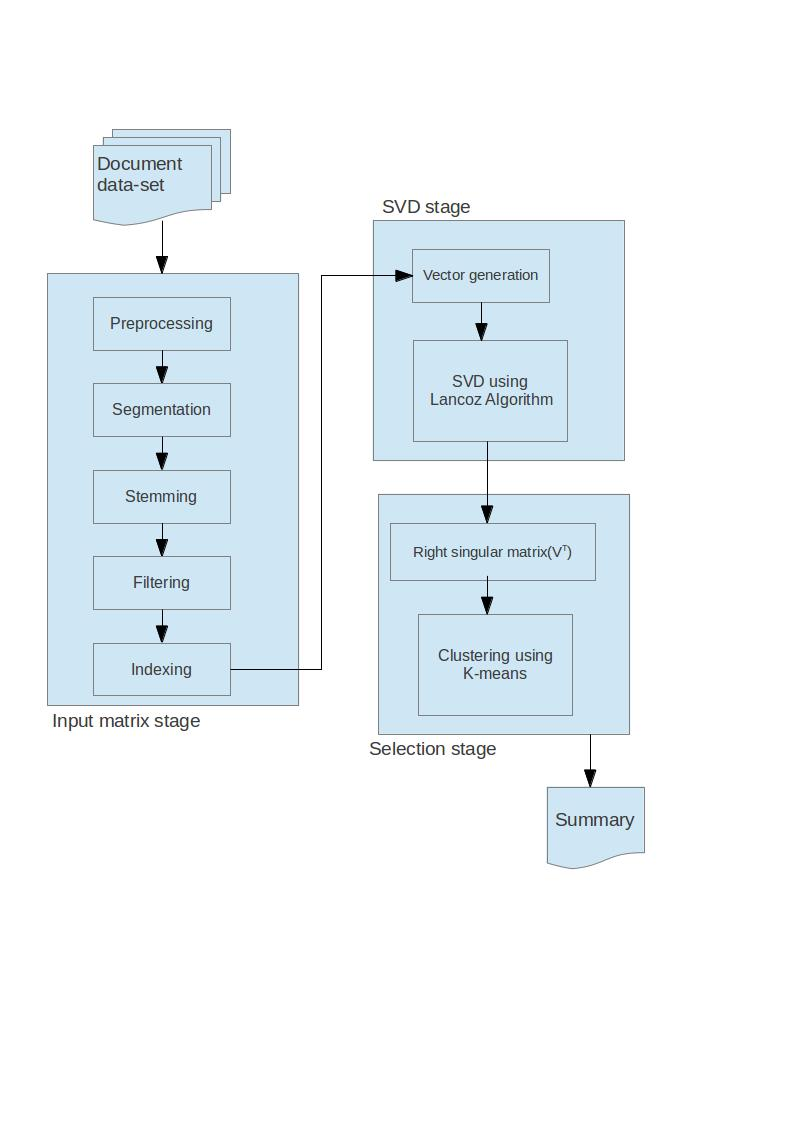
\includegraphics[width=0.5\textwidth]{design.jpg}
    \caption{System Design.}
\end{figure}
\section{Input matrix generation}
In the input matrix generation phase, The input is text dataset which has to be summarized and the intermediate output is
a sparse tf-idf matrix.
\subsection{Dataset}
Datasets for text summarization have to match certain criteria, the datasets publicly available and specific news related
datesets do not provide content redundancy. Handling redundancy in documents is an important feature in our system. For this reason
we use Apache Nutch,~\cite{nutch} an open-source web search engine to get similar datasets on a specific topic. Using nutch, we crawl the web
and fetch content from blogs, articles and websites related to the topic. The segments obtained from the crawler are parsed and the required
text is extracted. Content obtained from web can be in different formats like .pdf, .txt, .html, raw text is extracted from these file formats using
Tika~\cite{tika}.
\subsection{TF-IDF matrix}
Lucene API supports indexing of text in different formats like .html, .txt, several other document formats.
Preprocessing will involve removal of html tags, extraction of text from different formats, and conversion of text from different
languages to unicode. Segmentation of content is done based on groups of phrases, collection of sentences or single sentences. 
It is known that usage of single sentences provides better results. In this project, we will segment text based on senteces.
Using different segmentation methods will affect the nature of matrix, i.e., it will be sparse or dense. Word grouping is done through 
stemming where words like ``running,'' ``runner,'' ``run'' are considered as ``run''.
Using lucene API, words and sentences are filtered to match pre-defined criteria.
Lucene is used to index terms in each sentence. Lucene stores meta-data from documents in the form of 
key-value pairs, where key is the term and value is number of times it occurs in the sentence. Information related to sentences is
provided in the index.
The output of this phase is tf-idf sparse matrix which will be used for SVD.
\section{SVD on input matrix}
In this phase, SVD is used on the input matrix to obtain feature-sentence relation.
\subsection{SVD using Mahout}
Mahout API provides access to machine learning algorithms, which can be run on hadoop framework to parallelize the jobs.
Indexed terms from each sentence are converted to vectors based on a selected weighting metric (\textit{tf-idf, tf, log-entropy}).
Lancoz algorithm which is used for eigen value decomposition is modified to obtain SVD term vectors and extracted 
features-sentences matrix ($V^T$).In the sentence selection, the extracted $V^T$ matrix is used against different metrics to obtain
different sentence selection processes. Some of the procedures followed in this report are clustering using K-Means, Extracted sentence threshold.
Based on different sentence selection approaches we end up with different group of sentences being included into the summary.
\subsection{Parallelization strategy}
Right and left singular eigen vectors can be obtained from  matrix A by matrix multiplication $A A^T$, $A^T A$ respectively.
If A is not a square matrix, a few optimizations have to be done to make it a square matrix. Matrix multiplication can be parallelized
very effectively as a specific row does not have dependency over other rows or columns. Map-reduce framework will be used to
parallelize the indexing of documents and the lancoz algorithm. As most of the underlying algorithms, be it Lancoz, matrix multiplication,
KMeans clustering all of these are modified to take advantage of hadoop framework.
\section{Evaluation}
The obtained summary from system has to be evaluated against proven metrics and models to determine the quality compared to required standards.
A summary can be categorized as good one if it reflects the tone and content of the original report. In this system, we evaluate the obtained
summary against ROUGE-N, ROUGE-LCS and Tesla summarization metrics. Each of these metrics compares the extracted summary against summaries extracted by 
humans. Rouge-N and Tesla are N-gram based recall measures and ROUGE-LCS uses longest common subsequence of extracted words for benchmarking.
Detailed explanation of the metrics is provided in chapter 4. Analysis.
\section{Computation resources}
For better performance, speed and consistency, experiments were run on Amazon EC2 AMIs.
All the experiments had been conducted on Ubuntu 12.04 LTS (precise), and host will have minimum memory of 6GB.
Performance and speed of algorithms on multiple EC2 instances has been studied.
